\section{Structure}
\label{section:hybrid-cloud-structure}

    \autoref{figure:mw-reference-arch} shows a visual representation of the proposed hybrid cloud IIoT reference architecture. At first glance, we can see that the system is designed as a three-tier architecture, similar to the design in the IIRA in \autoref{subsubsection:iira}. These ``tiers'' will be referred to as ``environments'' from now on. The reference architecture describes the three tiers as ``edge'', ``fog'' and ``cloud'' environments, whereas each environment plays specific roles in processing data and control flows and has its own responsibilities. Note that the public literature often refers to the edge environment as the ``far edge'' and the fog tier as the ``near edge''. We can also see that all environments are based on the orchestration tool Kubernetes (see \autoref{section:orchestration-scheduling}) which results in having a uniform technology across the whole system. Let us take a look at the responsibilities of each environment now.

    
    \begin{figure}[htbp]
        \centering
        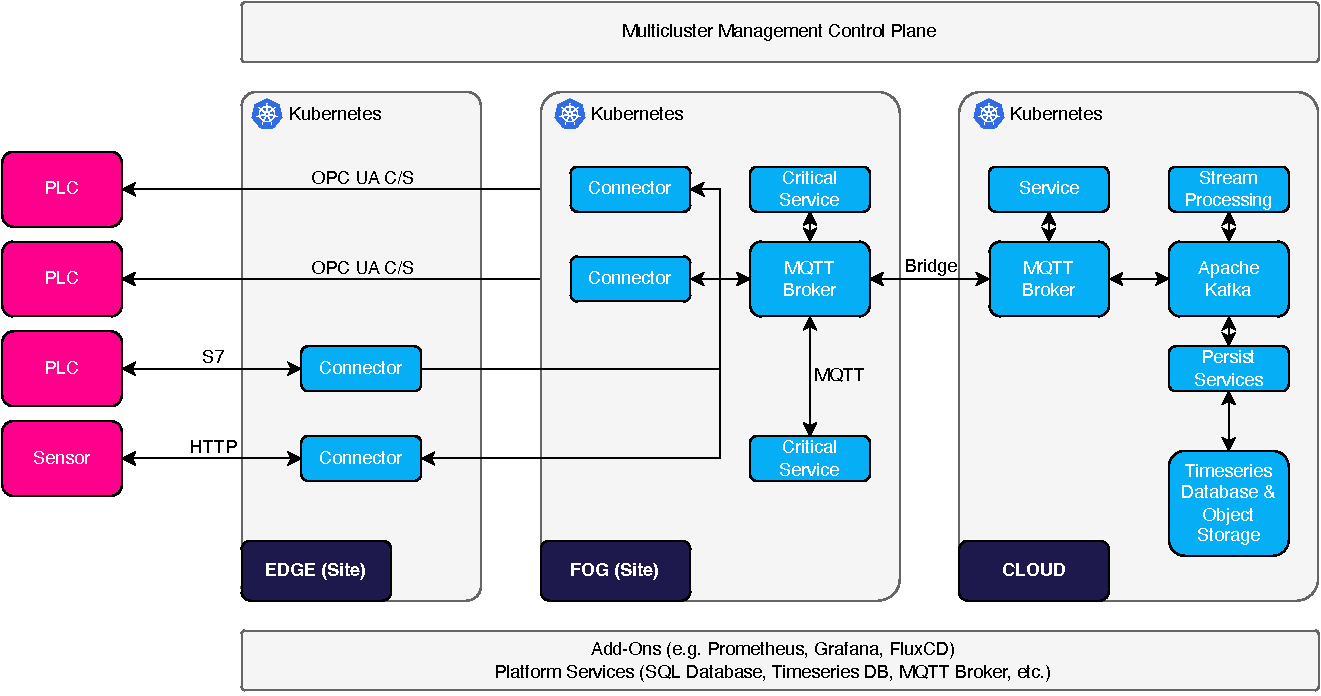
\includegraphics[width=\textwidth]{img/reference-architecture-bold.pdf}
        \caption{Hybrid Cloud IIoT Architecture by MaibornWolff GmbH \cite{building_iiot}}
        \label{figure:mw-reference-arch}
    \end{figure}

    \noindent The edge environment is the closest environment to the actual production site. It can exist many times per site and is mainly used for edge computing, which is especially relevant for low-latency workloads like visual inspection with machine learning, where latencies could cause damage to both humans and the production site. An edge environment typically consists of a bare-metal edge device running a single-node Kubernetes cluster, where an edge-optimized distribution of Kubernetes is used (\autoref{section:orchestration-scheduling}). Typical edge computing use cases include data preprocessing like aggregation, which is useful for countering high sampling rates that typically are an issue in IIoT systems or simple data analytics. Another very common use case for the edge environment is running adapter/connector services for IIoT components like sensors or PLCs that do not natively support the central communication protocol - in this case MQTT (see \autoref{subsubsection:mqtt}) - where the adapter service performs a protocol translation e.g.\ from Bluetooth Low Energy or LoRa over to MQTT. One scenario where such connectors are required is when common industry standards dealing with security and compliance like the cybersecurity norm ``IEC62443'' are enforced. In this norm, the segmentation of networks based on principles like least privilege, i.e. limiting the amount of network participants with access to data as much as possible, is required. A practical application of this in the real world happens when dealing with the S7 protocol, which is very common in the OT world and transmits data without any encryption. Following the cybersecurity norm, communication is then only allowed between communication partners that reside in the same network segment \cite{geiger_zones_2018}. An edge device in the same network segment as the IIoT device (e.g.\ a PLC) can be used to receive and send data via the unencrypted S7 protocol and forward it into other network segments using an encrypted protocol thus being compliant with the IEC62443 norm.  

    The successor of the edge environment is the fog environment, often referred to as the near-edge. It typically exists once per production site and consists of a highly available Kubernetes cluster running on bare-metal servers or virtual machines. It serves as the optimal environment for workloads that demand latency levels less stringent than those on the edge, yet more critical than those in the cloud.  Apart from typical data aggregation or analytics use cases, this environment houses production critical services. Since the environment runs fully on-premises, operability even during internet outages is guaranteed. The fog environment collects data from and sends data to all edge environments in the same site and communicates bi-directionally with the cloud environment. Unlike implementations following the IIoT reference architectures by cloud providers (\autoref{subsection:cloud-ref}) running services that require data from the whole factory before it hits the cloud with delay is easily feasible with this architecture. Similar to edge environments, having data just in an on-premises system also solves some confidentiality issues, e.g.\ by preprocessing data before storing it in the cloud or by just having stronger network security. Finally, the fog environments host MQTT brokers (\autoref{subsubsection:mqtt}). The MQTT broker in this environment is the central communication medium in the production site and should thus be deployed in a highly available fashion. The fog environment is also the default environment for machine connection to IoT-ready devices, which in our case means devices with support for MQTT, that directly send their data to this MQTT broker. Devices that need adapters for protocol translation from a protocol that is encrypted like OPC-UA to the MQTT standard can send their data to connector/adapter services which then forward the translated data to the broker. Devices that communicate using unencrypted protocols must send their data to a connector/adapter service in the edge environment, which then yet again forwards data to the MQTT broker. We will discuss the MQTT brokers further in \autoref{section:unified-namespace}.

    The third and last environment is the cloud environment which only exists once per IIoT system following this reference architecture. It will typically consist of a Kubernetes cluster managed by a cloud provider and a set of other supporting cloud resources. In this environment, typical domain services that have more relaxed requirements regarding latency and confidentiality are deployed. Access to the managed resources of cloud providers like databases, data/stream analytics, machine learning or storage enables developers to build services at an enormous scale. 
    Infrastructure services, which the cloud provider does not offer as managed resources, can be efficiently operated within the managed Kubernetes cluster, offering significant scalability. Because of the high amount of computational power, the cloud environment is also ideal for shared services like running CI/CD agents, hosting a private Git instance or having a central command \& control system with capabilities like observability (\autoref{section:observability}) and multi-cluster management (\autoref{section:multicluster-mgmt}) for operating the growing amount of environments. Apart from shared services, the cloud environment hosts the central MQTT broker, which all MQTT brokers in the fog environments communicate with, exchanging their data bi-directionally. We will discuss this MQTT broker as well in \autoref{section:unified-namespace}. \newline

    Note that this reference architecture is just a base recommendation and must be adjusted according to the requirements of the project. For example while \autoref{figure:mw-reference-arch} shows an instance of the distributed event streaming platform ``Apache Kafka'' in the cloud environment, Kafka can also be deployed in the fog environment of a site if the functionality is required there as well. Also while the architecture suggests using MQTT as the central protocol that also bridges data between fog environments and the cloud, it is absolutely possible to use Kafka for this functionality, if it is necessary for fulfilling the requirements of the system in question. Being able to schedule any workload on all environments is mainly possible due to the central orchestration technology Kubernetes (\autoref{section:orchestration-scheduling}) which is the basis of all environments and creates a uniform, homogeneous and highly flexible system. While different Kubernetes distributions like an edge-optimized distribution on edge and fog environments and a managed solution in the cloud environment are used in practice, the environments still offer a uniform set of interfaces for systems or humans to interact with \cite{building_iiot}. \newpage
